The UR20 has a system to practically create a single interface between the robot and PLC, in order to enhance the capabilities and functions of the cobot

\begin{figure}[h!]
	\centering
 	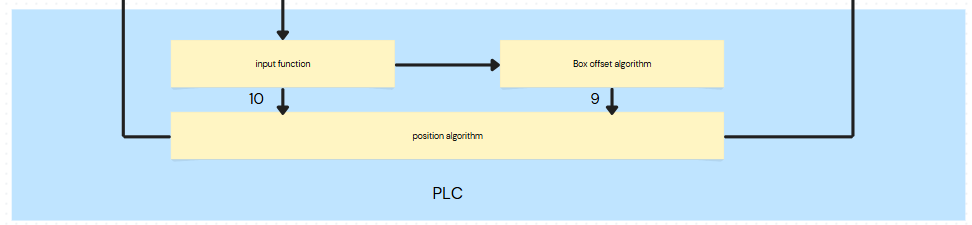
\includegraphics[width=0.60\textwidth]{images/Plc}
 \caption{PLC }
\end{figure}

\subsection{Input function}
The input function would be the readings of the environment knowing the positions of the pallet and reading the incoming box QR code 

\subsubsection{Assumptions}
Assumptions for the input function is that the boxes would have a visible QR code for sensor to read thus orientation of the box to be predefined. 

\subsubsection{Responsibilities}
The responsibitilies of the input fuction is soley to gather data that the PLC placement algorithm will use to preform its next action. such as the QR of the next box, the current state of the pallet, the location of any other nearby objects or people for safety concerns.

\subsubsection{Subsystem Interfaces}

\begin {table}[H]
\caption {Input fuction interfaces} 
\begin{center}
    \begin{tabular}{ | p{1cm} | p{6cm} | p{3cm} | p{3cm} |}
    \hline
    ID & Description & Inputs & Outputs \\ \hline
    \#01 & movement readings  & \pbox{3cm}{ destination\\position \\ speeds \\ safety sensor\\griper power} & \pbox{3cm}{formated data for PLC algorithm}  \\ \hline
    \#02 & box detection   & \pbox{3cm}{ QR reading\\position \\ speeds \\ safety sensor\\ griper power} & \pbox{3cm}{formated data for box offset algorithm }  \\ \hline
    
    \end{tabular}
\end{center}
\end{table}

\subsection{Box offset algorithm}
The box offset algorithm will be used to scan and determine the placement of the box 

\subsubsection{Assumptions}
QR codes will be used as a predefined locations for each bot and expected specfic order

\subsubsection{Responsibilities}
The responsibitilies of the placement function will be used to determine location of the box in the x,y,z dimentional plane and send it to the placement algorithm

\subsubsection{Subsystem Interfaces}


\begin {table}[H]
\caption {Box Offset algorithm interfaces} 
\begin{center}
    \begin{tabular}{ | p{1cm} | p{6cm} | p{3cm} | p{3cm} |}
    \hline
    ID & Description & Inputs & Outputs \\ \hline
    \#03 & movement  & \pbox{3cm}{QR reading\\position \\ speeds \\ safety sensor\\ griper power} & \pbox{3cm}{formated data for PLC algorithm }  \\ \hline
    
    \end{tabular}
\end{center}
\end{table}

\subsection{Placement algorithm }
The placement algorim is the central control of operations will tell the subsystems of the UR20 what actions to take given the output of the input function

\subsubsection{Assumptions}
The placement algorithm assumes that the gripper will have fixed strenght while moving a box and will be able to place without droping it. It expects belt and pallet location to be fixed and box orientation constant

\subsubsection{Responsibilities}
The responsibitilies of the placement function will be prefom send the appropriate values to the motors, in order to move arm to pick up the box then place it on pallet, and vacuum gripper to pick up and release the boxes. The algorithm will also be checking for safety based on the sensor to scan for people and stop or slow down movement.

\subsubsection{Subsystem Interfaces}


\begin {table}[H]
\caption {Placement algorithm interfaces} 
\begin{center}
    \begin{tabular}{ | p{1cm} | p{6cm} | p{3cm} | p{3cm} |}
    \hline
    ID & Description & Inputs & Outputs \\ \hline
    \#04 & movement  & \pbox{3cm}{QR reading\\destination\\ position \\ speeds \\ safety reading} & \pbox{3cm}{adjusted motor spreeds}  \\ \hline
    \#05 & gripper power  & \pbox{3cm}{destination\\postion} & \pbox{3cm}{ON/OFF}  \\ \hline
    
    \end{tabular}
\end{center}
\end{table}


